\section{Modification of the Christensen-Burley profile to better fit Monte
Carlo references}

The original formulation of the Christensen-Burley BSSRDF, first described in the
\cite{Burley:disney_siggraph15} and enhanced in \cite{Christensen:2015:ARP:2775280.2792555}, is
based on the fitting of the empirically chosen function to the Monte Carlo reference SSS renderings.
That function contains the sum of two exponentials, $1/r$ factor and the normalization coefficient
(equation \ref{eq:burley}):
\[ R_d(r) = As\dfrac{e^{-sr}+e^{-sr/3}}{8\pi r} \]

The exact form of scaling factor $s$ is also determined empirically. For searchlight configuration 
it has the form:
\begin{equation}
\label{eq:cb_scaling}
s=1.85-A + 7|A - 0.8|^3
\end{equation}

The results of my implementation of the original Christensen-Burley profile are shown as an example
of rendered sample at the figure \ref{fig:burley_searchlight_renders}. The corresponding plots are
provided at figure \ref{fig:burley_fitting}

\begin{figure}[h]
    \centering
    
\includegraphics[width=256pt,trim={0 0 256 0},clip]{imgs/renders/cb_montecarlo_slice}
    
\includegraphics[width=256pt,trim={0 0 256 0},clip]{imgs/renders/cb_modified_slice}
    
\includegraphics[width=256pt,trim={0 0 256 0},clip]{imgs/renders/cb_original_slice}
    \caption{Region of rendered image of Searchlight configuration. From top to bottom: Monte Carlo
    reference ($\sigma_a=0.01, \sigma_s=1.0$), modified Christensen-Burley, original
    Christensen-Burley ($A=0.89, s=0.975, t=19.2$)}
    \label{fig:burley_searchlight_renders}
\end{figure}

\begin{figure}[h]
    \centering
    \begin{subfigure}{\textwidth}
        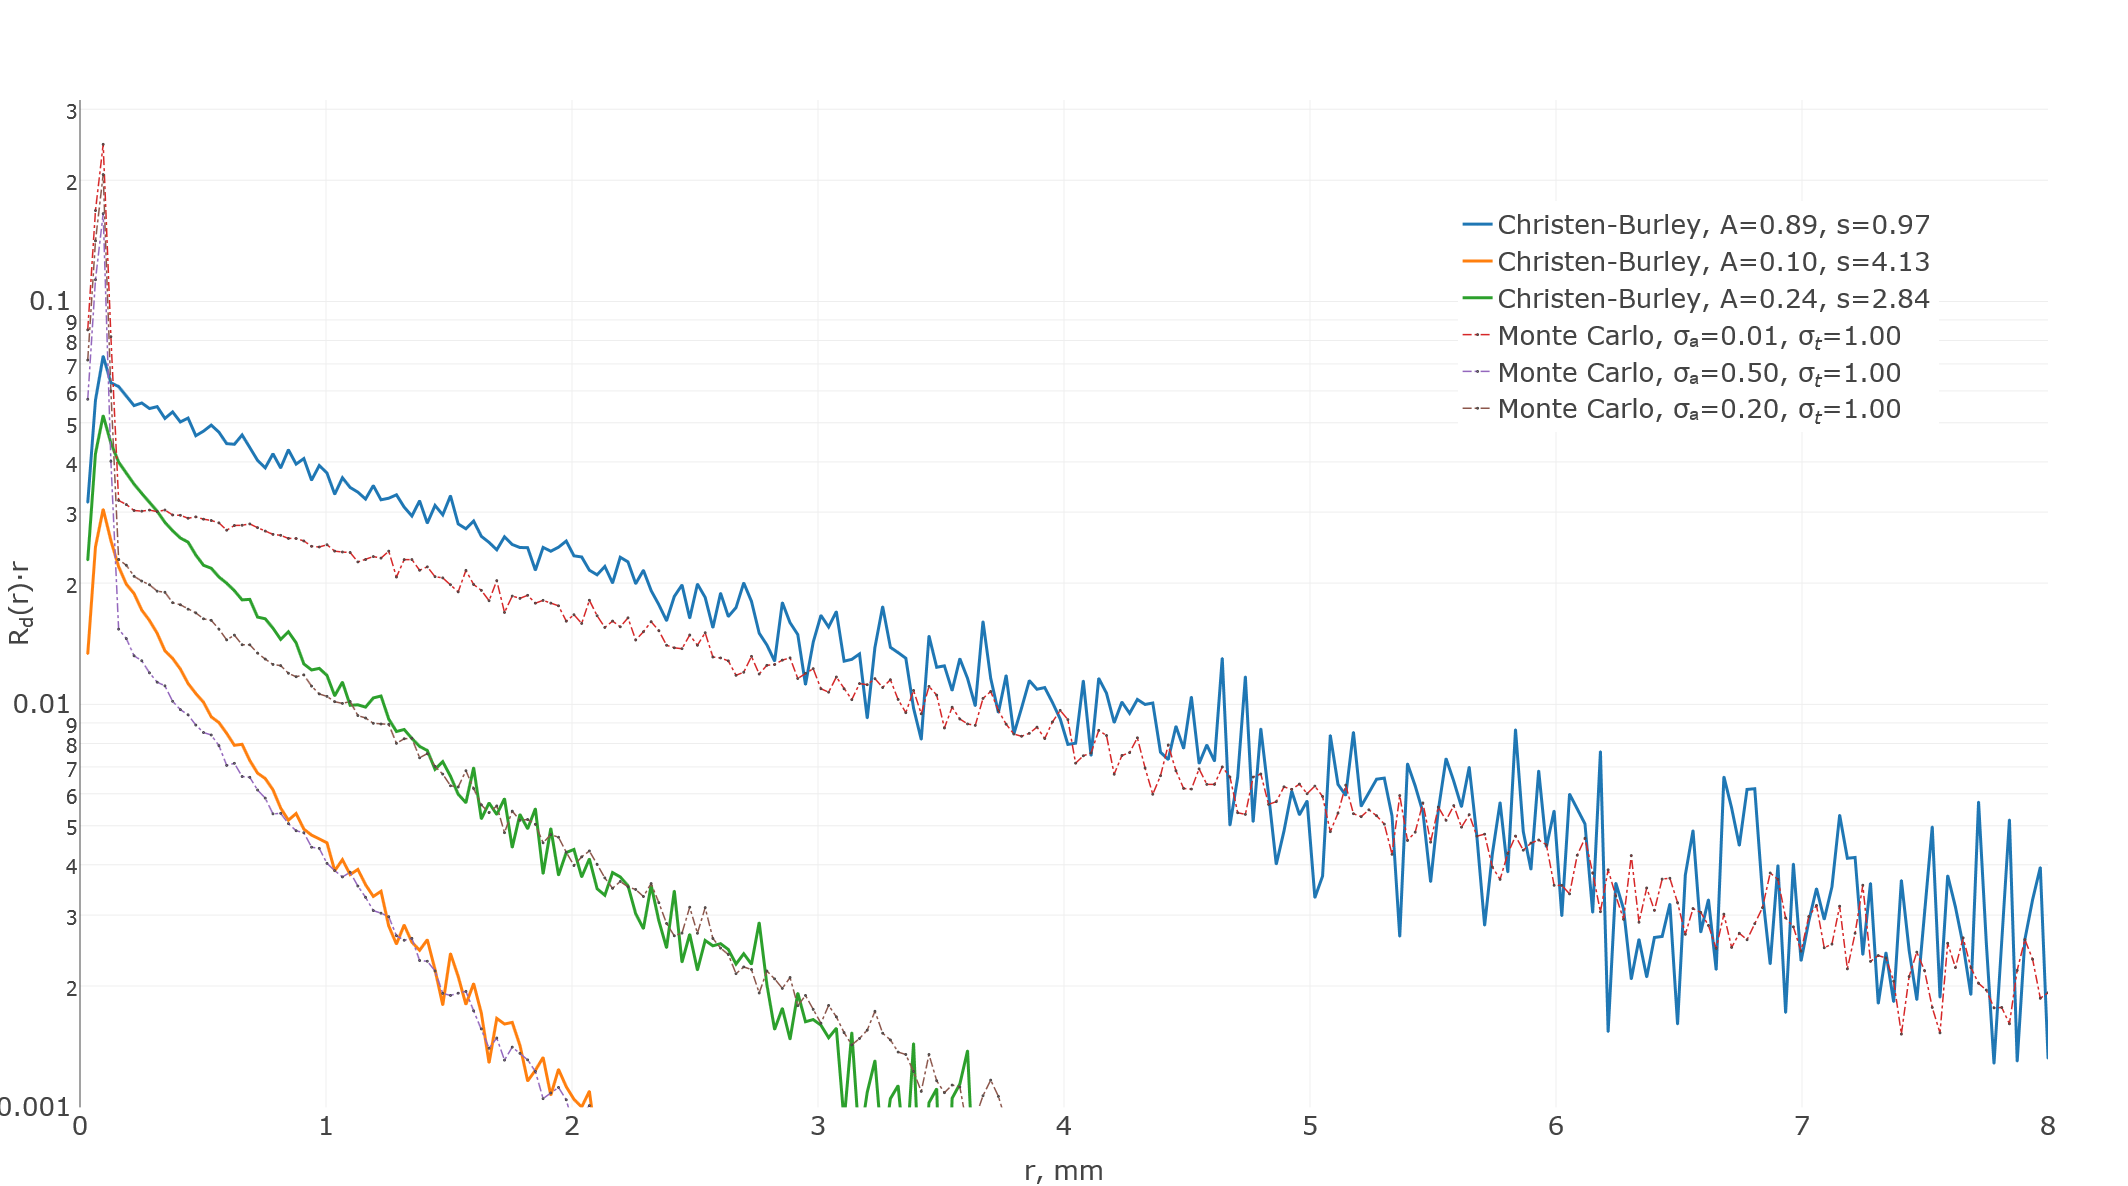
\includegraphics[width=\textwidth]{imgs/plots/cb_original_fitting}
        \caption{Original Christensen-Burley over Monte Carlo reference}
    \end{subfigure}
    \begin{subfigure}{\textwidth}
        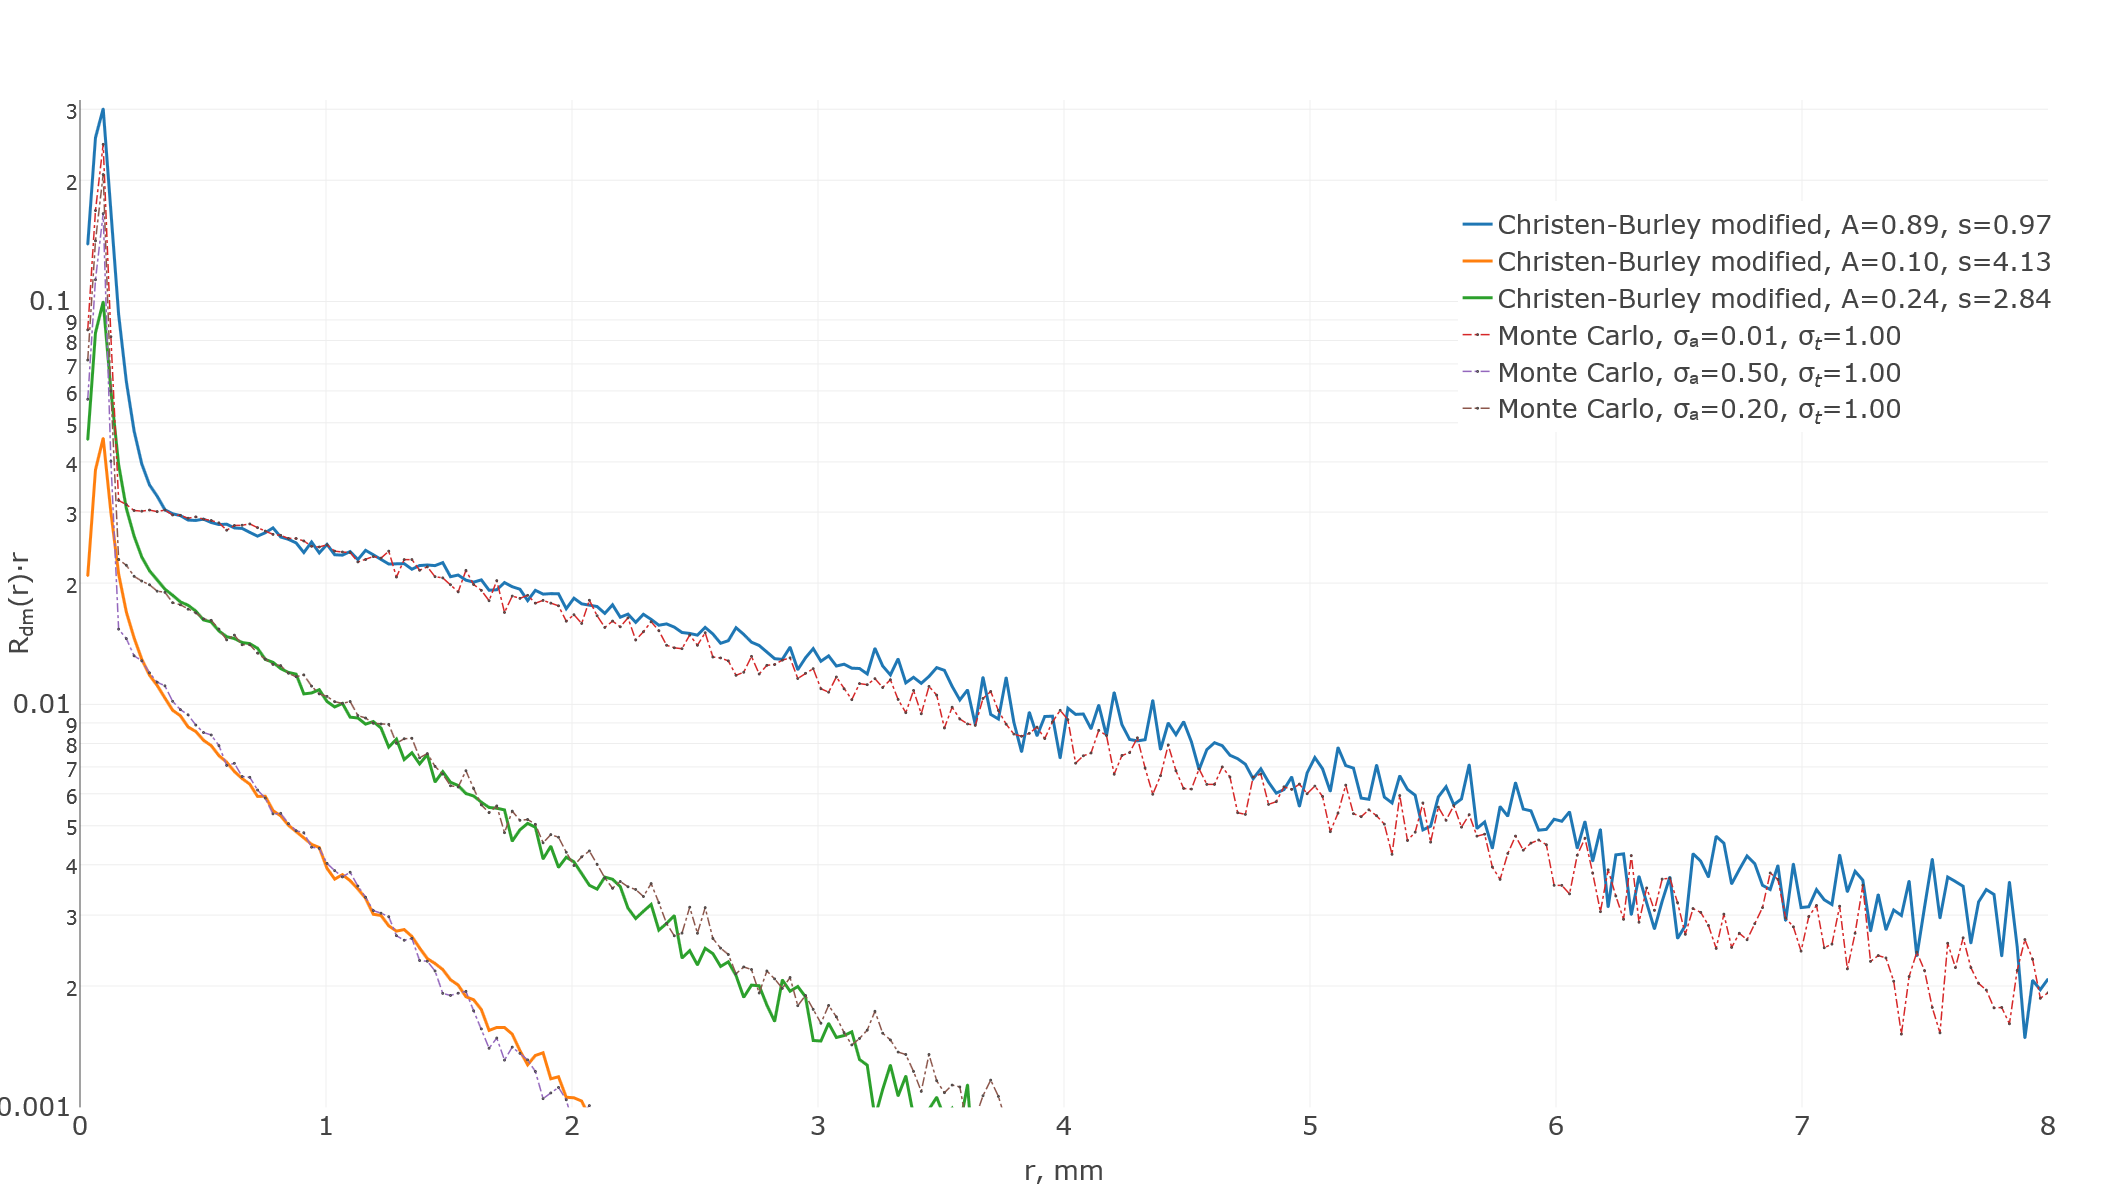
\includegraphics[width=\textwidth]{imgs/plots/cb_modified_fitting}
        \caption{Modified Christensen-Burley over Monte Carlo reference}
    \end{subfigure}

    \caption{Comparison between the original and proposed techniques in log-y
    scale. Monte Carlo references are in thin lines. The parameters $A$ and $s$ of the model are
    computed according to the method described in section \ref{section:cb_parametrization}}
    \label{fig:burley_fitting}
\end{figure}

As we can see from the plots \ref{fig:burley_fitting}, there is a tendency for
the original model to overestimate outgoing radiant exitance in the region close
to the light source. It is also noticeable as a an extra blurriness of the corresponding
lower rendered stripe at \ref{fig:burley_searchlight_renders}. This trend was observed in many
experiments with different optical properties of the material.

The proposed model to improve the Christensen-Burley BSSRDF profile includes the splitting of the
scaling parameter $s$ and using two different factors for each of the exponents:
\begin{equation}
\label{eq:burley_modified}
R_{dm}(r) = A\dfrac{te^{-tr}+se^{-sr/3}}{8\pi r}
\end{equation}

This modification allows to control the weight the exponents independent of each other and adjust
the profile to better match the corresponding Monte Carlo reference. The particular form of $s$ and
$t$ is based on the original function developed by Burley and Christensen. The coefficient $s$ of
the proposed model has the same form as the original equation (\ref{eq:cb_scaling}). But the form of
$t$ is adjusted with the multiplication of the linear function:
\begin{equation}
\label{eq:cb_scaling_modified}
t=s(20A+2)=(1.85-A + 7|A - 0.8|^3)(20A+2)
\end{equation}

The result of such modification and the comparison to the original profile is shown at figures
\ref{fig:burley_fitting} and \ref{fig:burley_searchlight_renders}.

We can observe that the modified BSSRDF has a better match to the Monte Carlo references for
materials with various albedo A. This effect appears as a distinct sharper gradient on the rendered
stripes.

\subsection{Notice about Monte Carlo references}
The brute force Monte Carlo integrators like unidirectional path tracer are used as a reference
implementation in this thesis. Although, the correctness and the comparison of this kind of
reference to the real-world measurements are not discussed.

Nevertheless, there are consistent results achieved for Searchlight experiment and other rendering
experiments of simple geometric shapes between different implementations of Monte Carlo integrators.
Three independently developed approaches were compared:
\begin{enumerate}
  \item Unidirectional path tracing integrator in P2 (see overview in section
  \ref{section:framework})
  \item Next Event Estimation integrator in P2 (see overview in section \ref{section:framework}
  \item Mitsuba Volumetric Path Tracer \cite{Mitsuba}
\end{enumerate}

All three methods produce the same result in the scope of their capabilities within the equivalent
scenes. This fact give us assurance of the correctness of the Monte Carlo algorithms which are
used as the references.
